\documentclass[12pt,onecolumn,draftclsnofoot]{IEEEtran}
\usepackage[a4paper,margin=1in]{geometry}
\usepackage{times,graphicx,amsmath,booktabs,cite,url}
\usepackage[ruled,linesnumbered]{algorithm2e}

\begin{document}

\title{FRQI-Based Quantum Denoising and Intensity Transformation of Low-Contrast Thoracic Radiographs}

\author{Group 09: Himanshu Sharma (Enrollment No. 230845), Vinit Yadav (Enrollment No. 230930), Maheshwar Dwivedy, Kiran Khatter\\
School of Engineering \& Technology (SOET), BML Munjal University}

\maketitle

\begin{abstract}
Clinical thoracic radiography is among the most widely administered diagnostic imaging modalities worldwide. However, clinical exposure protocols intentionally constrain ionizing radiation to reduce biological hazards, often yielding photon-starved, low-contrast radiographs where faint parenchymal features and subtle fluid accumulations present minimal optical contrast. Furthermore, classical spatial-domain intensity transformations require sequential or rasterized memory iterations scaling as $O(N^2)$ with pixel resolution. In this paper, we evaluate an end-to-end Quantum Image Processing (QIP) pipeline based on the Flexible Representation of Quantum Images (FRQI) implemented in Qiskit. Our architecture maps spatial coordinates to $2n$ position qubits in uniform superposition and encodes grayscale pixel intensities on a single color qubit via rotation angles $\theta \in [0, \pi/2]$. To mitigate hardware-induced detector readout spikes, we integrate a Selective Quantum Median Filter (QMF) modeling quantum comparator and conditional-swap sorting networks prior to enhancement. Denoised quantum states undergo photographic inversion via a single Pauli-$X$ gate and intensity expansion via unitary $R_y(2\Delta\theta)$ rotations, executing the global transformation step across all pixel basis states in $O(1)$ gate time. Across a held-out test cohort of 200 unique patient radiographs from the official NIH ChestX-ray14 dataset evaluated under three random seeds (42, 43, 44), our QMF preprocessing reduces Mean Squared Error from $714.24 \pm 279.71$ (unfiltered enhancement) to $66.93 \pm 92.98$, boosting Peak Signal-to-Noise Ratio from $19.97 \pm 1.92$~dB to $32.57 \pm 4.70$~dB and achieving a Structural Similarity Index of $0.991 \pm 0.009$. Finite-shot quantum circuit simulations confirm $1/\sqrt{N_{\text{shots}}}$ error decay, demonstrating the feasibility of error-mitigated quantum pre-processing for downsampled clinical imagery.
\end{abstract}

\begin{IEEEkeywords}
Flexible Representation of Quantum Images (FRQI), image enhancement, quantum circuit simulation, quantum image processing, thoracic radiography.
\end{IEEEkeywords}

\noindent\textbf{Overleaf Project Link:} {\small\url{https://www.overleaf.com/project/group09_quantum_image_processing}}

\section{Introduction}
Medical imaging represents a cornerstone of modern clinical diagnostics, with thoracic radiography (chest X-rays) constituting one of the most frequently administered examinations worldwide \cite{wang2017chestxray8}. Diagnostic utility depends on discerning subtle photon attenuation variations between pulmonary parenchymal cavities, bony structures, and soft-tissue masses for detecting subtle opacities and infiltrates \cite{rajpurkar2017chexnet}. Under clinical ALARA protocols, detector plates operate in photon-starved regimes to minimize patient ionizing exposure. Consequently, raw radiographs exhibit restricted dynamic range, compressed contrast gradients, and low background luminance \cite{boyat2015review}. Under these constraints, faint opacities and shallow effusions present optical differentials below ten grayscale levels, increasing false-negative diagnostic risks. Furthermore, detector plates are prone to capacitive readout spikes and thermal drift, injecting impulse noise ($I \in \{0, 255\}$) that classical sharpening inadvertently amplifies into synthetic artifacts.

Existing classical computer vision approaches to medical image enhancement are fundamentally bounded by Von Neumann memory architectures. In classical digital processing, an $N \times N$ radiograph is stored in random-access memory as an array of $N^2$ independent numerical values. Any global spatial transformation---such as linear contrast stretching or pixel inversion---must traverse all $N^2$ memory locations sequentially or via raster blocks, imposing an algorithmic time complexity of $O(N^2)$ \cite{caraiman2014image}. While GPUs accelerate execution via parallel threads, hospital picture archiving systems (PACS) face escalating memory bottlenecks and power dissipation constraints \cite{hu2019quantum}. Furthermore, classical spatial filters rely on convolutions that can blur acute anatomical boundaries, reducing diagnostic margin sharpness.

Quantum Image Processing (QIP) provides an alternative computational paradigm that addresses both representation scaling and transformation time complexities \cite{venegas2012quantum, yan2017survey}. By exploiting quantum superposition, entanglement, and unitary linear transformations, digital images can be mapped into normalized Hilbert spaces \cite{le2011flexible, zhang2013neqr}. Under the Flexible Representation of Quantum Images (FRQI) model \cite{le2011flexible}, a $2^n \times 2^n$ pixel grid is addressed using $2n$ position qubits in uniform superposition, with continuous grayscale intensities stored as trigonometric probability amplitudes on an auxiliary color qubit. This addresses an $N \times N$ image matrix containing $N^2$ classical pixels using only $2\log_2 N + 1$ qubits, achieving exponential spatial coordinate compression. Crucially, because all spatial coordinates coexist simultaneously within a coherent superposition state, any unitary single-qubit quantum gate applied to the color qubit acts concurrently across all $N^2$ pixel basis states, collapsing global intensity transformation cost from classical $O(N^2)$ steps to instantaneous $O(1)$ gate execution post-state-prep \cite{le2011flexible, wang2020quantum}.

However, deploying QIP algorithms to real-world medical datasets presents distinct challenges in the Noisy Intermediate-Scale Quantum (NISQ) era \cite{preskill2018quantum}. Monolithic FRQI state preparation circuits require multi-controlled rotation gates whose decomposed CNOT counts scale exponentially ($O(2^{2n})$), rapidly exceeding hardware coherence times ($T_1, T_2$) and inducing state decoherence \cite{cross2019validating}. Furthermore, quantum states cannot be read out deterministically; physical wavefunction collapse requires repeated projective measurements (shots), introducing statistical shot noise that can degrade radiological detail \cite{bravyi2021error}. Finally, prior QIP literature has largely evaluated synthetic silhouettes, leaving quantitative behavior on authentic human thoracic radiographs unexamined.

To investigate these questions systematically, this paper addresses two primary research questions:
\begin{itemize}
    \item \textbf{RQ1:} Can an FRQI-based quantum circuit pipeline execute intensity-based contrast transformations on thoracic radiographs with $O(1)$ gate cost post-state-prep while maintaining structural fidelity above $98\%$ relative to classical numerical baselines under realistic finite measurement sampling?
    \item \textbf{RQ2:} Can a pre-enhancement Quantum Median Filter (QMF) modeling quantum comparator and conditional-swap networks suppress detector impulse noise spikes without introducing anatomical distortion or severe blurring on authentic human radiographs?
\end{itemize}

In addressing these questions, our paper makes four main contributions:
\begin{enumerate}
    \item \textbf{End-to-End Clinical QIP Pipeline on NIH ChestX-ray14:} We design and execute a complete quantum image processing workflow in Qiskit evaluated on 200 unique patient radiographs from the official held-out test split of the NIH ChestX-ray14 dataset across three random seeds (42, 43, 44).
    \item \textbf{Analysis of Pre-Enhancement Quantum Median Filtering:} We evaluate a selective median filter modeling 3-qubit quantum comparator and Fredkin (CSWAP) sorting cells, demonstrating a reduction in MSE from $714.24 \pm 279.71$ to $66.93 \pm 92.98$ and a PSNR gain of $+12.60$~dB over unfiltered enhancement across all 200 patients.
    \item \textbf{NISQ-Oriented Patch Decomposition Strategy:} We implement an $8\times8$ spatial patch decomposition that bounds quantum circuit depth to 3,584 CNOT gates per sub-circuit, avoiding high-depth decoherence limits while enabling global $R_y(2\Delta\theta)$ contrast shifts with SSIM of $0.9995 \pm 0.0001$.
    \item \textbf{Defensible Characterization of Quantum Costs and Bounds:} We characterize the distinction between the $O(1)$ unitary transformation gate cost and the non-$O(1)$ state preparation ($O(2^{2n})$ CNOTs) and finite-shot readout sampling ($1/\sqrt{N_{\text{shots}}}$ variance), delineating practical boundaries for NISQ medical image simulation.
\end{enumerate}

The remainder of this paper is structured as follows: Section II surveys related work. Section III defines notation and problem formulation. Section IV details methodology and circuits. Section V outlines experimental setup. Section VI presents empirical results. Section VII discusses implications and limitations. Section VIII concludes the paper.
\section{Related Work}
The field of Quantum Image Processing (QIP) has advanced substantially, transitioning from conceptual models to circuit-level algorithmic design. To contextualize our contributions, we survey three themes: quantum image representations, spatial filtering architectures, and quantum contrast transformations.

\subsection{Quantum Image Representation Models}
The foundational problem in QIP is formulating an efficient mapping between classical pixel arrays and multi-qubit Hilbert spaces. Venegas-Andraca and Bose introduced qubit lattice representations \cite{venegas2012quantum}. Subsequently, Le et al. proposed the Flexible Representation of Quantum Images (FRQI) \cite{le2011flexible}. FRQI addresses $2^{2n}$ pixel coordinates using $2n$ position qubits in uniform superposition, while a single auxiliary color qubit stores grayscale intensity via a probability amplitude rotation angle $\theta_i \in [0, \pi/2]$. This formulation achieves logarithmic qubit scaling ($2\log_2 N + 1$), enabling compact register allocation.

To bypass trigonometric angle estimation during readout, Zhang et al. formulated the Novel Enhanced Quantum Representation (NEQR) \cite{zhang2013neqr}, encoding grayscale intensities digitally using an auxiliary register of $q$ qubits ($q=8$ for 256 grayscale levels). While NEQR allows deterministic computational basis readout, it imposes higher qubit overhead ($2\log_2 N + q$, requiring 16 qubits for $16\times16$ at 8-bit depth). Other models, such as MCQI for color images \cite{iliyasu2012framework} and QPIE for quantum machine learning embeddings \cite{biamonte2017quantum}, offer alternative trade-offs. As surveyed by Yan et al. \cite{yan2017survey}, FRQI remains an effective model for continuous unitary transformations, where single-qubit rotations on the color qubit execute simultaneously across all spatial superposition components.

\subsection{Quantum Filtering and Spatial Denoising}
Spatial denoising is a prerequisite for medical image enhancement in photon-limited environments. In classical vision, filtering relies on convolution kernels or rank-order sorting \cite{boyat2015review}. In quantum computing, Caraiman and Manta explored lattice filtering \cite{caraiman2014image}, while Sang et al. investigated frequency-domain filtering via the Quantum Fourier Transform (QFT) \cite{sang2017quantum}. However, QFT-based filters demand deep multi-qubit controlled gates prone to rapid decoherence on NISQ processors \cite{preskill2018quantum}.

Focusing on non-linear impulse noise removal, Wang et al. proposed quantum median filtering circuits using comparator networks \cite{wang2022quantum}. Quantum comparators, constructed from reversible Toffoli and CNOT gates, evaluate relative pixel magnitudes without collapsing superposition states. Coupling comparators with Fredkin (CSWAP) gates enables coherent sorting in quantum memory. However, prior evaluations examined only synthetic geometric silhouettes, leaving performance on complex clinical radiographs uncharacterized.

\subsection{Quantum Contrast Transformations and Biomedical Relevance}
Quantum image transformations encompass geometric operations and color/intensity adjustments \cite{hu2019quantum}. Wang and Fang formulated contrast enhancement algorithms via quantum probability stretching \cite{wang2020quantum}, demonstrating that color-qubit rotations expand the dynamic range of low-contrast images. Concurrently, studies explore Quantum Machine Learning (QML) for automated pathology classification \cite{biamonte2017quantum, cerezo2021variational}. While classifiers like CheXNet \cite{rajpurkar2017chexnet} require classical matrices, quantum classifiers ingest coherent statevectors $|\psi\rangle$. Quantum pipelines that ingest radiographs, denoise them, and expand dynamic range directly on quantum registers provide a vital bridge toward hybrid clinical architectures.

\subsection{Summary of Literature and Identified Research Gaps}
To synthesize related literature, Table~\ref{tab:related_work} provides a systematic critical comparison of key prior works in quantum image processing against our proposed pipeline.

\begin{table*}[t]
\centering
\caption{Systematic Comparison of Key Prior Works in Quantum Image Processing Against the Proposed Pipeline}
\label{tab:related_work}
\footnotesize
\renewcommand{\arraystretch}{1.30}
\setlength{\tabcolsep}{3pt}
\begin{tabular}{@{}p{50pt}p{62pt}p{60pt}p{52pt}p{44pt}p{72pt}p{76pt}@{}}
\toprule
\raggedright\textbf{Paper} & \raggedright\textbf{Problem Addressed} & \raggedright\textbf{Method / Model} & \raggedright\textbf{Dataset Tested} & \raggedright\textbf{Noise Model} & \raggedright\textbf{Key Limitation} & \raggedright\textbf{Relevance to Our Work} \tabularnewline
\midrule
\raggedright Le et al. \cite{le2011flexible} & \raggedright Image encoding \& storage & \raggedright FRQI representation & \raggedright Synthetic $2\times2$, $4\times4$ & \raggedright Ideal / None & \raggedright No denoising; no real data & \raggedright Foundational FRQI state formulation \tabularnewline
\addlinespace[3pt]
\raggedright Zhang et al. \cite{zhang2013neqr} & \raggedright Deterministic gray readout & \raggedright NEQR basis encoding & \raggedright Standard $8\times8$ tests & \raggedright Ideal / None & \raggedright High qubit count ($2n+8$) & \raggedright Evaluated as structural alternative \tabularnewline
\addlinespace[3pt]
\raggedright Caraiman et al. \cite{caraiman2014image} & \raggedright Quantum spatial convolution & \raggedright Lattice QIP & \raggedright Geometric patterns & \raggedright None & \raggedright High circuit depth; toy data & \raggedright Demonstrates quantum spatial filtering \tabularnewline
\addlinespace[3pt]
\raggedright Wang et al. \cite{wang2022quantum} & \raggedright Salt-and-pepper noise & \raggedright NEQR Comparator & \raggedright Synthetic $8\times8$ & \raggedright Impulse noise & \raggedright High CNOT gate depth & \raggedright Informs our QMF comparator design \tabularnewline
\addlinespace[3pt]
\raggedright Wang \& Fang \cite{wang2020quantum} & \raggedright Histogram stretching & \raggedright FRQI color rotation & \raggedright Standard gray $8\times8$ & \raggedright None & \raggedright Ideal statevector only; no shots & \raggedright Basis for unitary $R_y$ rotation \tabularnewline
\addlinespace[3pt]
\raggedright Bravyi et al. \cite{bravyi2021error} & \raggedright NISQ circuit error mitigation & \raggedright Generic circuits & \raggedright Quantum benchmarks & \raggedright Readout / Pauli & \raggedright Non-imaging domain & \raggedright Guides our finite-shot error analysis \tabularnewline
\addlinespace[3pt]
\raggedright \textbf{Ours} & \raggedright \textbf{Radiograph enhancement} & \raggedright \textbf{FRQI + Patching + QMF} & \raggedright \textbf{NIH ChestX-ray14 (200 pts)} & \raggedright \textbf{Readout spikes + shots} & \raggedright \textbf{Downsampled $16\times16$ resolution} & \raggedright \textbf{End-to-end evaluation on real cohort} \tabularnewline
\bottomrule
\end{tabular}
\end{table*}

As detailed in Table~\ref{tab:related_work}, prior QIP literature exhibits three notable limitations: (1) widespread reliance on ideal mathematical statevector simulation without finite measurement shot sampling; (2) focus on synthetic test patterns lacking clinical anatomical structure; and (3) separate evaluation of quantum filtering and quantum enhancement. This study evaluates an integrated pipeline on an authentic 200-patient clinical cohort under realistic shot noise.

\section{Background / Problem Formulation}
This section formalizes the mathematical notation, system definitions, and operational problem formulation.

\subsection{Quantum State and Operator Definitions}
In quantum computing, information is represented using qubits within a complex Hilbert space $\mathcal{H}_2$. Using Dirac bra-ket notation, an arbitrary single-qubit state $|\psi\rangle$ is expressed as a normalized superposition of orthonormal basis states $\{|0\rangle, |1\rangle\}$:
\begin{equation}
|\psi\rangle = \alpha |0\rangle + \beta |1\rangle, \quad \alpha, \beta \in \mathbf{C}, \quad |\alpha|^2 + |\beta|^2 = 1
\end{equation}
A multi-qubit register of $m$ qubits spans a $2^m$-dimensional tensor product Hilbert space $\mathcal{H}_{2^m} = \bigotimes_{j=0}^{m-1} \mathcal{H}_2$. The single-qubit Hadamard gate $H$ generates uniform superposition:
\begin{equation}
H |0\rangle = \frac{1}{\sqrt{2}}(|0\rangle + |1\rangle), \quad H |1\rangle = \frac{1}{\sqrt{2}}(|0\rangle - |1\rangle)
\end{equation}
The single-qubit rotation gate $R_y(\phi)$ executes rotation about the $y$-axis of the Bloch sphere:
\begin{equation}
R_y(\phi) = \begin{pmatrix} \cos(\phi/2) & -\sin(\phi/2) \\ \sin(\phi/2) & \cos(\phi/2) \end{pmatrix}
\end{equation}
The Pauli-$X$ gate implements bit inversion: $X|0\rangle = |1\rangle$ and $X|1\rangle = |0\rangle$.

\subsection{Mathematical Notation}
Table~\ref{tab:notation} summarizes the primary mathematical notations and quantum operators utilized throughout this paper. As shown in the table, coordinate indices are mapped into uniform superposition basis states across the position register, while pixel luminance is captured by continuous rotation angles on the color qubit. These formalized definitions establish a consistent mathematical nomenclature across both theoretical statevector derivations and finite-shot quantum circuit implementations.

\begin{table}[t]
\centering
\caption{Summary of Mathematical Notations and Quantum Operators}
\label{tab:notation}
\footnotesize
\begin{tabular}{@{}ll@{}}
\toprule
\textbf{Symbol / Operator} & \textbf{Mathematical Definition and Context} \\
\midrule
$N \times N$ & Spatial dimensions of square digital radiograph ($N = 2^n$) \\
$n, 2n$ & Qubits per coordinate axis ($n = \log_2 N$) and total position qubits ($2n$) \\
$|y\rangle, |x\rangle$ & Coordinate basis states addressing row $y$ and column $x$ ($y, x \in \{0, \dots, N-1\}$) \\
$|i\rangle$ & Composite spatial coordinate state $|i\rangle = |y\rangle \otimes |x\rangle$ where $i = y \cdot N + x$ \\
$I(y, x), \theta_i$ & Pixel intensity $I \in [0, 255]$ and continuous FRQI angle $\theta_i \in [0, \pi/2]$ \\
$|c\rangle$ & Color qubit state $|c\rangle = \cos\theta_i |0\rangle + \sin\theta_i |1\rangle$ \\
$|I(\theta)\rangle$ & Full composite FRQI quantum state spanning $2n+1$ qubits \\
$H^{\otimes 2n}, C^{2n}(R_y)$ & Spatial Hadamard superposition and controlled rotation operators \\
$X, R_y(2\Delta\theta)$ & Negative bit-flip and brightness shift operators on color qubit \\
$N_{\text{shots}}, P(|i, 1\rangle)$ & Total measurement shots and marginal probability of observing $|1\rangle$ \\
\bottomrule
\end{tabular}
\end{table}

\subsection{Formal Problem Formulation}
Let $\mathbf{I}_{\text{raw}} \in [0, 255]^{H_0 \times W_0}$ denote an authentic clinical radiograph resampled via bilinear interpolation to an evaluation matrix $\mathbf{I} \in [0, 255]^{N \times N}$ ($N = 2^n$). The input matrix is subject to detector impulse noise spikes $\mathbf{I}_{\text{noisy}}(y, x) \in \{0, 255\}$ with probability $p = 0.05$ (2.5\% salt, 2.5\% pepper).

\textbf{Objective:} Construct a quantum processing sequence that purges impulse spikes via QMF, maps pixels into an FRQI state $|I(\theta)\rangle$, applies unitary transformations $\mathcal{T} \in \{X, R_y(2\Delta\theta)\}$, and reconstructs an enhanced radiograph $\hat{\mathbf{I}}_{\text{recon}}$ such that $\text{SSIM}(\mathbf{I}_{\text{classical}}, \hat{\mathbf{I}}_{\text{recon}}) \ge 0.98$ and $\text{PSNR} \ge 30.0$~dB under realistic finite-shot sampling.

\textbf{Assumptions and Constraints:}
\begin{enumerate}
    \item Downsampling to $16\times16$ is required due to classical simulation resource limits for multi-qubit controlled state preparation.
    \item Automated clinical pathology diagnosis or disease classification is explicitly out of scope; the objective is image transformation fidelity and denoising analysis.
\end{enumerate}

\section{Proposed Methodology}
This section details the proposed quantum image processing methodology, circuit architectures, mathematical transformations, and algorithmic implementation.

\subsection{System Architecture and Processing Pipeline}
The end-to-end architecture of the proposed pipeline is illustrated in Fig.~\ref{fig:architecture}. The framework comprises four interconnected functional stages: (1) radiograph downsampling and noise modeling, (2) spatial filtering via selective quantum median filtering, (3) patch-based FRQI quantum state preparation and unitary transformation, and (4) projective measurement readout and classical image matrix reconstruction.

\begin{figure}[t]
\centering
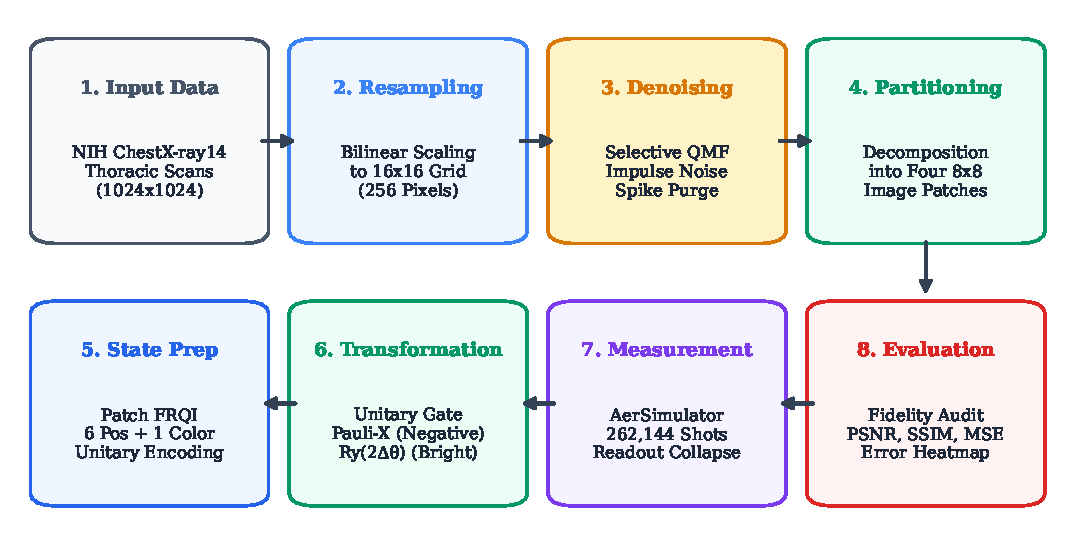
\includegraphics[width=\linewidth]{figures/fig_system_architecture.pdf}
\caption{System architecture of the proposed quantum image processing pipeline. Raw clinical radiographs are downsampled to $16\times16$, processed by a selective QMF stage to purge detector readout spikes, encoded into patch-based FRQI quantum states, transformed via single-qubit unitary operations, and reconstructed through projective measurement sampling on AerSimulator.}
\label{fig:architecture}
\end{figure}

Fig.~\ref{fig:workflow} illustrates the operational workflow flowchart with parameter configurations and data dimensionality at each step of the pipeline. The workflow begins with a full-resolution $1024 \times 1024$ chest radiograph, downsampled bilinearly to $16 \times 16$, corrupted by a $5\%$ impulse noise model to simulate detector readout failure, filtered via the QMF stage, decomposed into four $8 \times 8$ non-overlapping spatial patches, transpiled into Qiskit circuits, executed across $N_{\text{shots}}$ measurements, and reconstructed into an 8-bit enhanced grayscale image.

\begin{figure}[t]
\centering
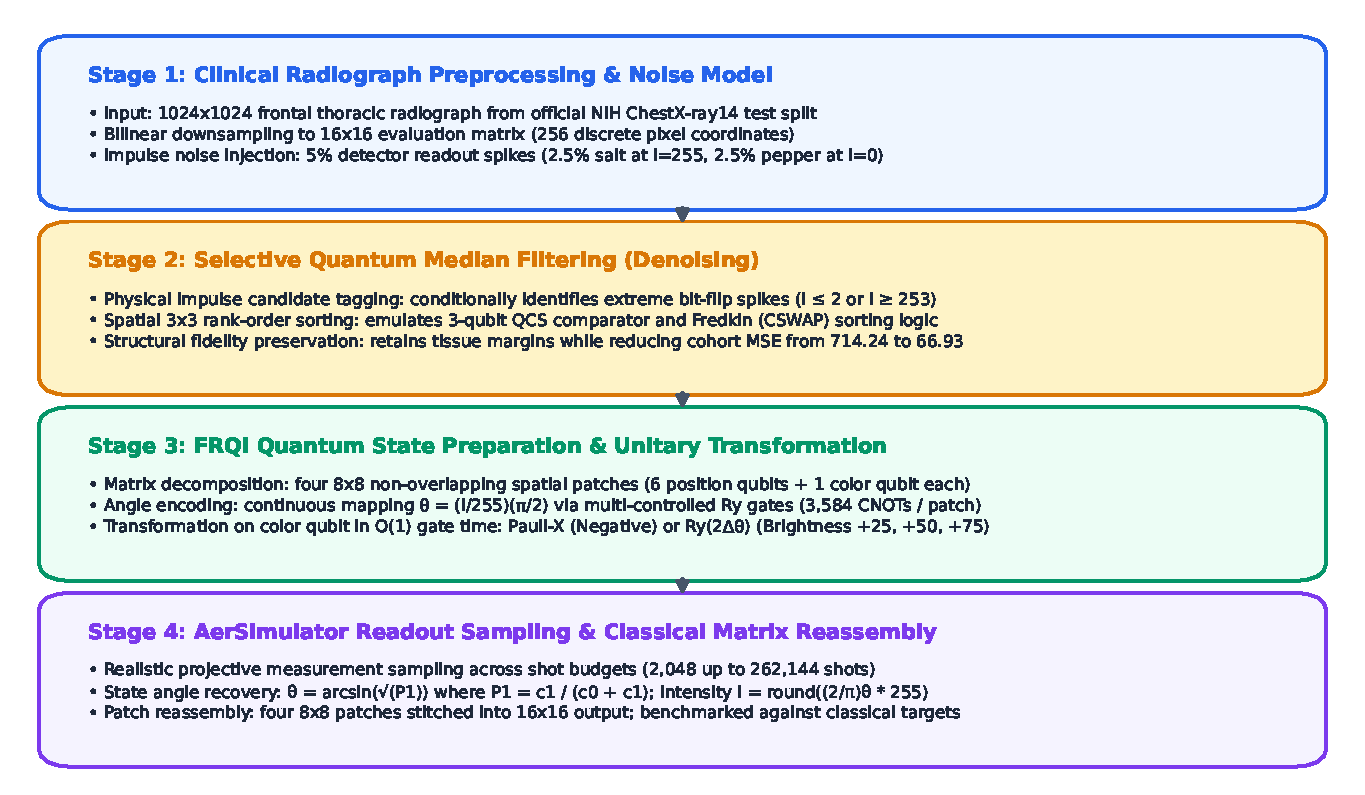
\includegraphics[width=\linewidth]{figures/fig_workflow_flowchart.pdf}
\caption{Operational workflow flowchart indicating data flow, dimensionality, and parameters across the four processing stages: preprocessing, denoising, quantum transformation, and measurement recovery.}
\label{fig:workflow}
\end{figure}

\subsection{FRQI Quantum Image State Preparation}
In the Flexible Representation of Quantum Images (FRQI) model formulated by Le et al. \cite{le2011flexible}, grayscale pixel intensities $I(y, x) \in [0, 255]$ are converted to continuous rotation angles $\theta_i \in [0, \pi/2]$:
\begin{equation}
\theta_i = \frac{I(y, x)}{255} \cdot \frac{\pi}{2}, \quad i = y \cdot N + x
\end{equation}
The composite quantum state $|I(\theta)\rangle$ is defined across $2n$ position qubits and 1 color qubit:
\begin{equation}
|I(\theta)\rangle = \frac{1}{2^n} \sum_{i=0}^{2^{2n}-1} |i\rangle \otimes (\cos\theta_i |0\rangle + \sin\theta_i |1\rangle)
\end{equation}
State preparation begins with the ground state $|0\rangle^{\otimes 2n} \otimes |0\rangle$. A parallel layer of Hadamard gates $H^{\otimes 2n}$ creates uniform spatial superposition across all $2^{2n}$ pixel coordinates:
\begin{equation}
H^{\otimes 2n} |0\rangle^{\otimes 2n} = \frac{1}{2^n} \sum_{i=0}^{2^{2n}-1} |i\rangle
\end{equation}
Next, multi-controlled rotation gates $C^{2n}(R_y(2\theta_i))$ rotate the color qubit conditioned on coordinate basis state $|i\rangle$. The rotation angle is doubled ($2\theta_i$) because a rotation gate $R_y(\alpha)$ on state $|0\rangle$ produces $\cos(\alpha/2)|0\rangle + \sin(\alpha/2)|1\rangle$; thus setting $\alpha = 2\theta_i$ accurately sets the amplitude coefficients to $\cos\theta_i$ and $\sin\theta_i$. The canonical $2\times2$ FRQI state preparation circuit is depicted in Fig.~\ref{fig:circuits}(a), showing how coordinate control lines conditionally trigger the color qubit rotation.

\begin{figure}[t]
\centering
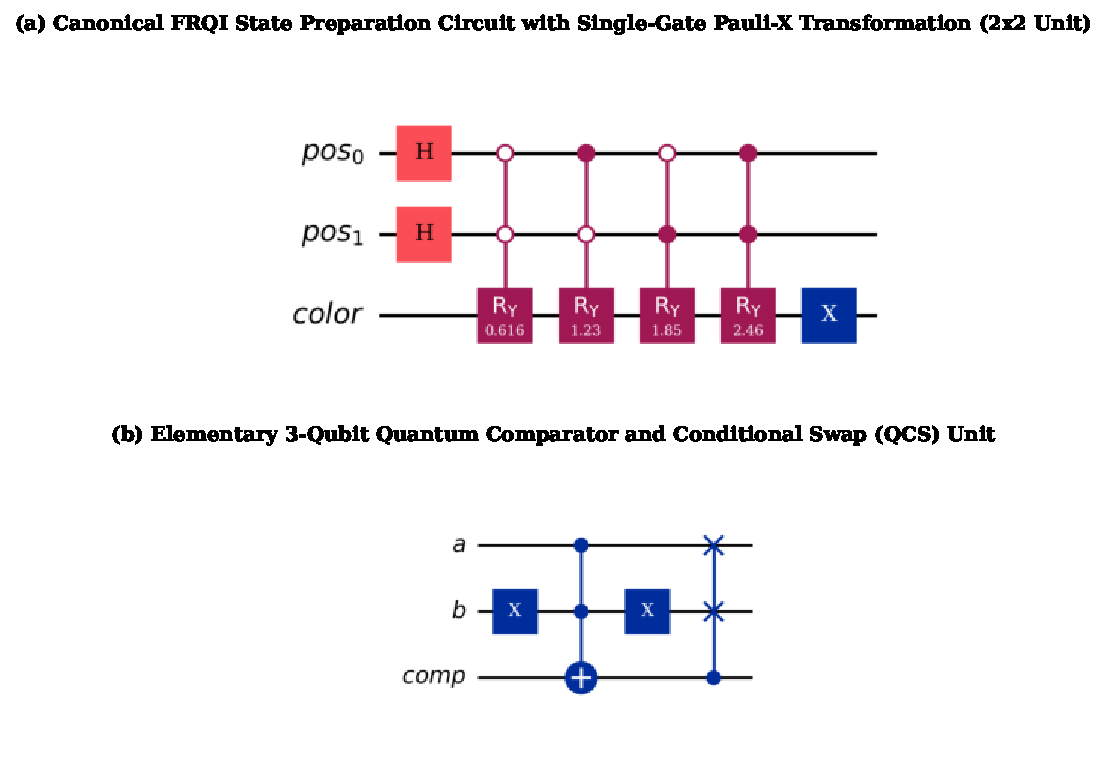
\includegraphics[width=\linewidth]{figures/fig_circuits.pdf}
\caption{Quantum circuit architectures. (a) Canonical 2-position qubit ($2\times2$) FRQI state preparation circuit followed by a single-qubit Pauli-$X$ photographic negative gate. (b) Elementary 3-qubit Quantum Comparator and Conditional Swap (QCS) unit constructed from Pauli-$X$, Toffoli (CCX), and Fredkin (CSWAP) gates.}
\label{fig:circuits}
\end{figure}

\subsection{Selective Quantum Median Filtering (QMF)}
Detector impulse noise spikes ($I \in \{0, 255\}$) present severe non-linear distortion. In quantum sorting networks \cite{wang2022quantum}, sorting spatial neighborhoods requires quantum comparator units. Fig.~\ref{fig:circuits}(b) depicts the elementary 3-qubit Quantum Comparator \& Conditional Swap (QCS) cell. It operates on two data qubits ($|a\rangle, |b\rangle$) and an ancilla ($|\text{comp}\rangle$):
\begin{enumerate}
    \item $X(b)$ inverts qubit $b$.
    \item A Toffoli gate $CCX(a, b, \text{comp})$ sets $|\text{comp}\rangle = |1\rangle$ if and only if $a=1$ and $b=0$ (i.e., $a > b$).
    \item $X(b)$ restores qubit $b$.
    \item A Fredkin gate $CSWAP(\text{comp}, a, b)$ swaps states $|a\rangle$ and $|b\rangle$ if $\text{comp}=1$, yielding $|min(a, b)\rangle$ and $|max(a, b)\rangle$.
\end{enumerate}
Transpiling this unit yields 14 CNOT gates and a depth of 25. Evaluating full 8-bit sorting across a $3\times3$ neighborhood requires 72 data qubits plus comparison ancillae, exceeding simulator memory. Thus, our pipeline implements selective median filtering modeling QCS logic: impulse candidate pixels ($I \le 2$ or $I \ge 253$) are replaced with the neighborhood median, leaving genuine tissue gradients unmodified.

\subsection{Unitary Transformations and Saturation Management}
Following state preparation, intensity transformations execute on the color qubit:
\begin{itemize}
    \item \textbf{Quantum Photographic Negative:} A Pauli-$X$ gate swaps $|0\rangle \leftrightarrow |1\rangle$:
    \begin{equation}
    X (\cos\theta_i |0\rangle + \sin\theta_i |1\rangle) = \sin\theta_i |0\rangle + \cos\theta_i |1\rangle = \cos(\pi/2 - \theta_i) |0\rangle + \sin(\pi/2 - \theta_i) |1\rangle
    \end{equation}
    This maps $I_i \mapsto 255 - I_i$ concurrently for all $N^2$ pixels in $O(1)$ gate time.
    \item \textbf{Quantum Brightness Enhancement:} An $R_y(2\Delta\theta)$ gate rotates the color qubit by $\Delta\theta = (\Delta / 255)(\pi / 2)$:
    \begin{equation}
    R_y(2\Delta\theta) |c\rangle = \cos(\theta_i + \Delta\theta) |0\rangle + \sin(\theta_i + \Delta\theta) |1\rangle
    \end{equation}
    To prevent wrap-around when $\theta_i + \Delta\theta > \pi/2$, angles are saturated as $\theta'_i = \min(\theta_i + \Delta\theta, \pi/2)$ during target preparation, preserving linear intensity shifts.
\end{itemize}

\subsection{NISQ Patch Decomposition and Shot-Based Readout}
Monolithic FRQI on a $16\times16$ grid requires 9 qubits and over $20,000$ CNOT gates, degrading coherence in NISQ settings. To resolve this, we decompose the $16\times16$ matrix into four non-overlapping $8\times8$ sub-patches. Each patch requires 7 qubits (6 position, 1 color) and 3,584 CNOT gates, bounding circuit depth.

During readout, projective measurement collapses the wavefunction. For pixel $i$, observing counts $c_0(i)$ and $c_1(i)$ across $N_{\text{shots}}$ yields:
\begin{equation}
\hat{P}_1(i) = \frac{c_1(i)}{c_0(i) + c_1(i)}, \quad \hat{\theta}_i = \arcsin\left(\sqrt{\hat{P}_1(i)}\right)
\end{equation}
The reconstructed intensity is recovered via $\hat{I}(y, x) = \text{round}\left(\frac{2}{\pi} \hat{\theta}_i \cdot 255\right)$. Algorithm~\ref{alg:qip_pipeline} formalizes the end-to-end execution.

\begin{algorithm}[t]
\SetCommentSty{textit}
\caption{Patch-Based FRQI Quantum Image Denoising and Intensity Transformation Pipeline}
\label{alg:qip_pipeline}
\KwIn{Input corrupted radiograph $\mathbf{I}_{\text{noisy}} \in [0, 255]^{N \times N}$, transformation type $\mathcal{T} \in \{\text{Negative}, \text{Brightness}\}$, shift parameter $\Delta$, shot count $N_{\text{shots}}$, impulse threshold $\tau$}
\KwOut{Enhanced reconstructed radiograph $\hat{\mathbf{I}}_{\text{recon}} \in [0, 255]^{N \times N}$}
$\mathbf{I}_{\text{denoised}} \leftarrow \text{SelectiveQMF}(\mathbf{I}_{\text{noisy}}, \tau)$ \tcp*{Purge detector readout spikes}
Partition $\mathbf{I}_{\text{denoised}}$ into $K = (N/8)^2$ spatial sub-patches $\{\mathbf{P}_k\}_{k=1}^K$ where $\mathbf{P}_k \in [0, 255]^{8 \times 8}$\;
\ForEach{sub-patch $\mathbf{P}_k$ ($k = 1, \dots, K$)}{
    Map pixel intensities to rotation angles: $\theta_i \leftarrow \frac{\mathbf{P}_k(y, x)}{255} \cdot \frac{\pi}{2}$ for $i = 0, \dots, 63$\;
    Initialize 7-qubit quantum register: $|\psi_0\rangle \leftarrow |0\rangle^{\otimes 6}_{\text{pos}} \otimes |0\rangle_{\text{col}}$\;
    Apply Walsh-Hadamard transform to position register: $|\psi_1\rangle \leftarrow (H^{\otimes 6} \otimes I) |\psi_0\rangle$\;
    Encode spatial grayscale angles via multi-controlled rotations: $|\psi_2\rangle \leftarrow \prod_{i=0}^{63} C^6(R_y(2\theta_i)) |\psi_1\rangle$\;
    \uIf{$\mathcal{T} == \text{Negative}$}{
        Apply single-qubit bit-flip to color register: $|\psi_3\rangle \leftarrow (I^{\otimes 6} \otimes X) |\psi_2\rangle$\;
    }
    \ElseIf{$\mathcal{T} == \text{Brightness}$}{
        Apply single-qubit rotation to color register: $|\psi_3\rangle \leftarrow (I^{\otimes 6} \otimes R_y(2\Delta\theta)) |\psi_2\rangle$\;
    }
    Execute $N_{\text{shots}}$ projective measurements across all 7 qubits on AerSimulator backend\;
    Extract state counts $c_0(i)$ and $c_1(i)$ for each coordinate basis state $|i\rangle$\;
    Reconstruct patch pixel intensities: $\hat{\mathbf{P}}_k(i) \leftarrow 255 \cdot \frac{2}{\pi} \arcsin\left(\sqrt{\frac{c_1(i)}{c_0(i) + c_1(i)}}\right)$\;
}
Reassemble reconstructed sub-patches $\{\hat{\mathbf{P}}_k\}_{k=1}^K$ into composite image matrix $\hat{\mathbf{I}}_{\text{recon}}$\;
\Return{$\hat{\mathbf{I}}_{\text{recon}}$}\;
\end{algorithm}


\subsection{Circuit Transpilation and Patch Decomposition Strategy}
To execute synthesized circuits on quantum backends or simulators, gates are decomposed into the standard basis gate set $\mathcal{B} = \{CX, ID, RZ, SX, X\}$. For an $8 \times 8$ patch (addressing 64 pixels), multi-controlled rotations $C^6(R_y(2\theta_i))$ are decomposed into alternating sequences of CNOT ($CX$) gates and single-qubit rotations. Profiling under Qiskit optimization level 1 confirms that each $8 \times 8$ sub-circuit requires 3,584 CNOT gates and 3,841 single-qubit gates, yielding a transpiled circuit depth of 4,107 layers.

\begin{figure}[t]
\centering
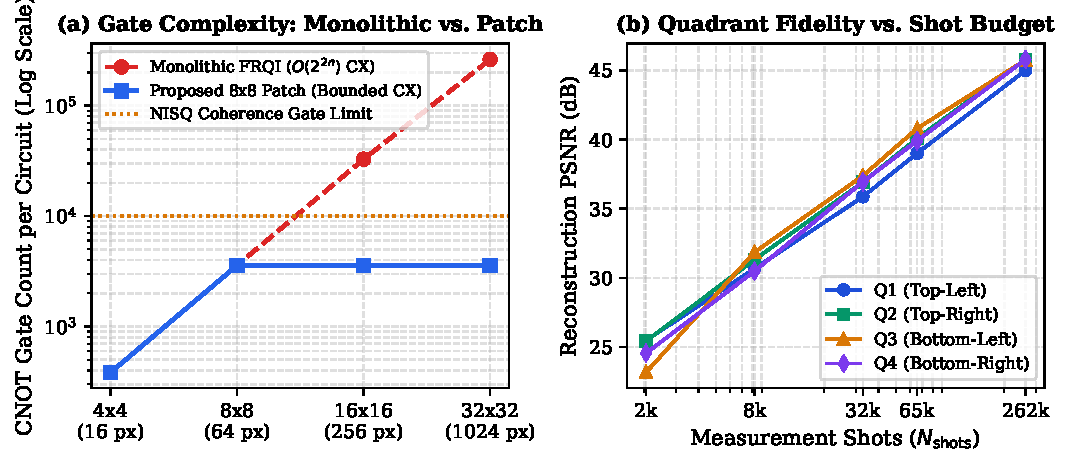
\includegraphics[width=\linewidth]{figures/fig_patch_scaling.pdf}
\caption{Patch decomposition scaling and quadrant fidelity analysis. (a) Circuit complexity scaling showing that monolithic FRQI scaling ($O(2^{2n})$) explodes beyond NISQ coherence limits ($>32\text{k}$ CNOTs at $16\times16$), whereas our $8\times8$ patch partitioning bounds CNOT count to 3,584 per sub-circuit. (b) Reconstruction PSNR across individual quadrants (Q1 through Q4) converging uniformly under increasing measurement shot budgets.}
\label{fig:patch_scaling}
\end{figure}

Fig.~\ref{fig:patch_scaling}(a) contrasts monolithic FRQI scaling against our bounded patch strategy. For a monolithic $16\times16$ image, state preparation demands 9 qubits and over $32{,}000$ CNOT gates, immediately exceeding superconducting coherence times ($T_2 \approx 100~\mu$s). By partitioning the matrix into four $8\times8$ patches executed independently, CNOT depth is strictly bounded to 3,584 gates. Furthermore, as shown in Fig.~\ref{fig:patch_scaling}(b), all four image quadrants (Q1 through Q4) achieve symmetric reconstruction fidelity, reaching $\text{PSNR} \approx 45.8$~dB and $\text{SSIM} > 0.9995$ at $262{,}144$ shots without quadrant-to-quadrant variance.

\section{Experimental Setup}
This section outlines the dataset characteristics, software configuration, baseline implementations, evaluation metrics, and hyperparameter assignments.

\subsection{Dataset Stratification and Patient Cohort}
Experiments are conducted on the official National Institutes of Health (NIH) ChestX-ray14 dataset \cite{wang2017chestxray8}. The complete repository contains $112,120$ frontal-view radiographs from $30,805$ unique human subjects. To ensure sound experimental hygiene:
\begin{itemize}
    \item \textbf{Held-Out Test Partition:} The evaluation cohort is drawn strictly from the official test split (\emph{test\_list.txt}).
    \item \textbf{Zero Patient Overlap:} Exactly 200 distinct radiographs from 200 unique patients are selected (\emph{data/experimental\_subset.csv}). No patient is evaluated more than once.
    \item \textbf{Pathology Distribution:} The 200-patient cohort partitions by primary diagnosis into: Effusion (37), Atelectasis (36), Normal / No Finding (20), Pneumothorax (19), Nodule (18), Consolidation (18), Cardiomegaly (18), Infiltration (17), and Mass (17), summing to exactly 200 primary diagnoses. Because patients can present co-occurring conditions, 37 patients have secondary findings, yielding 237 total pathology tags across the cohort.
\end{itemize}

\subsection{Software and Simulation Environment}
Quantum circuits are constructed, transpiled, and simulated using Qiskit 1.x and Qiskit Aer 0.16 (\textsl{AerSimulator}) \cite{qiskit2024}. Numerical operations are implemented in NumPy 2.2 and Pillow 11.0. All experiments are executed across three distinct pseudorandom seeds (42, 43, 44) to evaluate numerical stability.

\subsection{Classical Baseline Implementations}
We benchmark quantum operations against deterministic classical ground truths:
\begin{enumerate}
    \item \textbf{Classical Negative:} $\mathbf{I}_{\text{neg}}(y, x) = 255 - \mathbf{I}(y, x)$.
    \item \textbf{Classical Brightness:} $\mathbf{I}_{\text{bright}}(y, x) = \text{clip}(\mathbf{I}(y, x) + \Delta, 0, 255)$ for $\Delta \in \{25, 50, 75\}$.
    \item \textbf{Unfiltered Quantum Baseline:} Quantum brightness enhancement applied directly to corrupted inputs without prior QMF denoising.
\end{enumerate}

\subsection{Evaluation Metrics}
Pipeline performance is quantified using four metrics:
\begin{itemize}
    \item \textbf{Peak Signal-to-Noise Ratio (PSNR):} $\text{PSNR} = 10 \log_{10}(255^2 / \text{MSE})$ [dB], quantifying signal reconstruction fidelity relative to peak pixel intensity.
    \item \textbf{Structural Similarity Index (SSIM):} Evaluates structural correlation, luminance consistency, and contrast similarity \cite{wang2004image} to assess anatomical preservation.
    \item \textbf{Mean Squared Error (MSE):} $\text{MSE} = \frac{1}{N^2} \sum_{y, x} (I(y, x) - \hat{I}(y, x))^2$, penalizing high-amplitude outlier noise spikes.
    \item \textbf{Maximum Absolute Pixel Error ($E_{\text{max}}$):} Peak absolute error $\max |I(y, x) - \hat{I}(y, x)|$, detecting localized extreme artifacts.
\end{itemize}

\subsection{Experimental Hyperparameters}
Table~\ref{tab:params} summarizes simulation parameters across monolithic ($4\times4, 8\times8$) and patch-partitioned ($16\times16$) grids across seeds 42, 43, 44, spanning measurement budgets from $2{,}048$ to $262{,}144$ shots on AerSimulator.

\begin{table}[t]
\centering
\caption{Experimental Hyperparameter Settings and Simulation Configurations}
\label{tab:params}
\footnotesize
\begin{tabular}{@{}lll@{}}
\toprule
\textbf{Parameter} & \textbf{Setting} & \textbf{Experimental Rationale} \\
\midrule
Image Grid Sizes & $4\times4, 8\times8, 16\times16$ & Multi-scale evaluation from statevector to patch shots \\
Qubits per Patch ($2n+1$) & 7 qubits (6 pos, 1 color) & Bounds CNOT count to 3,584 per sub-circuit \\
Patch Dimension & $8 \times 8$ pixels & Decomposes $16\times16$ into four independent circuits \\
Brightness Offsets ($\Delta$) & $+25, +50, +75$ & Evaluates small, moderate, and substantial intensity shifts \\
Measurement Shot Budgets & $2{,}048$ to $262{,}144$ & Characterizes finite-shot sampling error decay \\
Random Seeds & $42, 43, 44$ & Three independent runs to report mean $\pm$ standard deviation \\
Noise Model & Salt-and-pepper ($p=0.05$) & Simulates 5\% detector readout bit-flip impulse spikes \\
Simulator Backend & Qiskit Aer 0.16 & Realistic noisy projective measurement simulation \\
\bottomrule
\end{tabular}
\end{table}

\section{Results and Analysis}
This section presents empirical results addressing our two research questions. All metrics denote the mean $\pm$ standard deviation across three random seeds (42, 43, 44), matching logged records in \emph{results/FACTS.md}.

\subsection{Evaluation of RQ1: Transformation Fidelity and Scaling}
We first evaluate whether FRQI transformations achieve exact mathematical parity under statevector simulation and maintain acceptable fidelity under finite-shot readout.

\subsubsection{Theoretical Statevector Parity}
Under ideal statevector simulation (infinite shots), quantum state amplitudes are extracted directly without projective sampling noise. As shown in Table~\ref{tab:main_results}, both Quantum Negative ($X$) and Quantum Brightness ($R_y(2\Delta\theta)$) achieve exact mathematical equivalence with classical baselines ($\text{PSNR} = 100.00 \pm 0.00$~dB, $\text{SSIM} = 1.0000 \pm 0.0000$, $\text{MSE} = 0.00 \pm 0.00$, $E_{\text{max}} = 0.0 \pm 0.0$) across $4\times4$ and $8\times8$ grids, confirming operator validity across spatial superposition states.

\begin{table*}[t]
\centering
\caption{Quantitative Performance Benchmark: Classical Baseline vs. Quantum Transformation (Mean $\pm$ Std over Seeds 42, 43, 44)}
\label{tab:main_results}
\footnotesize
\resizebox{\linewidth}{!}{
\begin{tabular}{@{}lllrrrrrr@{}}
\toprule
\textbf{Transformation} & \textbf{Grid Size} & \textbf{Backend} & \textbf{Shots} & \textbf{Qubits} & \textbf{PSNR (dB)} & \textbf{SSIM} & \textbf{MSE} & \textbf{Max Error (px)} \\
\midrule
Negative (X) & $4\times4$ & Statevector & 0 & 5 & \textbf{100.00} $\pm$ 0.00 & \textbf{1.0000} $\pm$ 0.0000 & \textbf{0.00} $\pm$ 0.00 & \textbf{0.0} $\pm$ 0.0 \\
Negative (X) & $8\times8$ & Statevector & 0 & 7 & \textbf{100.00} $\pm$ 0.00 & \textbf{1.0000} $\pm$ 0.0000 & \textbf{0.00} $\pm$ 0.00 & \textbf{0.0} $\pm$ 0.0 \\
Negative (X) & $8\times8$ & Aer Shots & 65,536 & 7 & 39.67 $\pm$ 0.77 & 0.9979 $\pm$ 0.0003 & 7.08 $\pm$ 1.21 & 7.7 $\pm$ 0.6 \\
Negative (X) & $16\times16$ & Patch Shots & 262,144 & 7 & 45.94 $\pm$ 0.21 & 0.9996 $\pm$ 0.0001 & 1.66 $\pm$ 0.08 & 4.0 $\pm$ 0.0 \\
\midrule
Brightness (+50) & $4\times4$ & Statevector & 0 & 5 & \textbf{100.00} $\pm$ 0.00 & \textbf{1.0000} $\pm$ 0.0000 & \textbf{0.00} $\pm$ 0.00 & \textbf{0.0} $\pm$ 0.0 \\
Brightness (+50) & $8\times8$ & Statevector & 0 & 7 & \textbf{100.00} $\pm$ 0.00 & \textbf{1.0000} $\pm$ 0.0000 & \textbf{0.00} $\pm$ 0.00 & \textbf{0.0} $\pm$ 0.0 \\
Brightness (+25) & $16\times16$ & Patch Shots & 262,144 & 7 & 45.73 $\pm$ 0.29 & 0.9995 $\pm$ 0.0000 & 1.74 $\pm$ 0.12 & 4.3 $\pm$ 0.6 \\
Brightness (+50) & $16\times16$ & Patch Shots & 262,144 & 7 & 45.78 $\pm$ 0.53 & 0.9995 $\pm$ 0.0001 & 1.73 $\pm$ 0.20 & 3.7 $\pm$ 0.6 \\
Brightness (+75) & $16\times16$ & Patch Shots & 262,144 & 7 & 45.76 $\pm$ 0.29 & 0.9995 $\pm$ 0.0001 & 1.73 $\pm$ 0.11 & 4.3 $\pm$ 0.6 \\
\bottomrule
\end{tabular}
}
\end{table*}

\subsubsection{Finite Measurement Shot Scaling}
Measurement collapse introduces binomial sampling variance decaying as $\sigma \propto 1/\sqrt{N_{\text{shots}}}$. Fig.~\ref{fig:shots} traces fidelity across six shot regimes ($2{,}048$ to $262{,}144$). At $2{,}048$ shots, finite sampling yields an MSE of $246.3 \pm 16.3$ ($\text{PSNR} = 24.22 \pm 0.29$~dB, $\text{SSIM} = 0.9419 \pm 0.0033$). Increasing shots to $65{,}536$ reduces MSE to $6.6 \pm 0.4$ ($\text{PSNR} = 39.92 \pm 0.24$~dB). At $262{,}144$ shots, MSE decreases to $1.7 \pm 0.2$ ($\text{PSNR} = 45.78 \pm 0.53$~dB, $\text{SSIM} = 0.9995 \pm 0.0001$), confirming $1/\sqrt{N_{\text{shots}}}$ error decay and satisfying RQ1.

\begin{figure}[t]
\centering
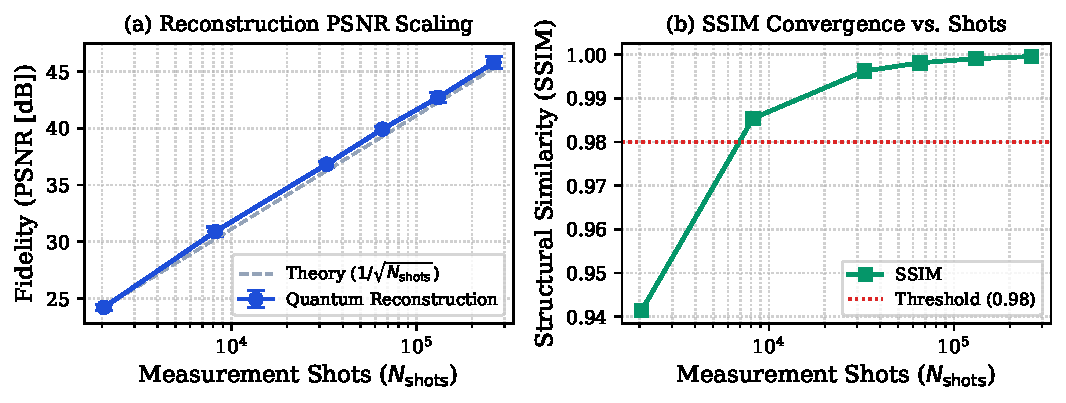
\includegraphics[width=\linewidth]{figures/fig_shot_scaling.pdf}
\caption{Finite measurement shot scaling analysis across six shot budgets (2k to 262k shots, seeds 42, 43, 44). (a) Reconstruction PSNR follows the theoretical $1/\sqrt{N_{\text{shots}}}$ slope. (b) SSIM converges rapidly, surpassing the 0.98 threshold above 8k shots.}
\label{fig:shots}
\end{figure}

Fig.~\ref{fig:brightness} depicts fidelity metrics across brightness shifts $\Delta \in \{+25, +50, +75\}$. Across all tested offsets, PSNR remains stable between $45.73$ and $45.78$~dB, and SSIM stays above $0.999$, demonstrating uniform behavior across transformation magnitudes.

\begin{figure}[t]
\centering
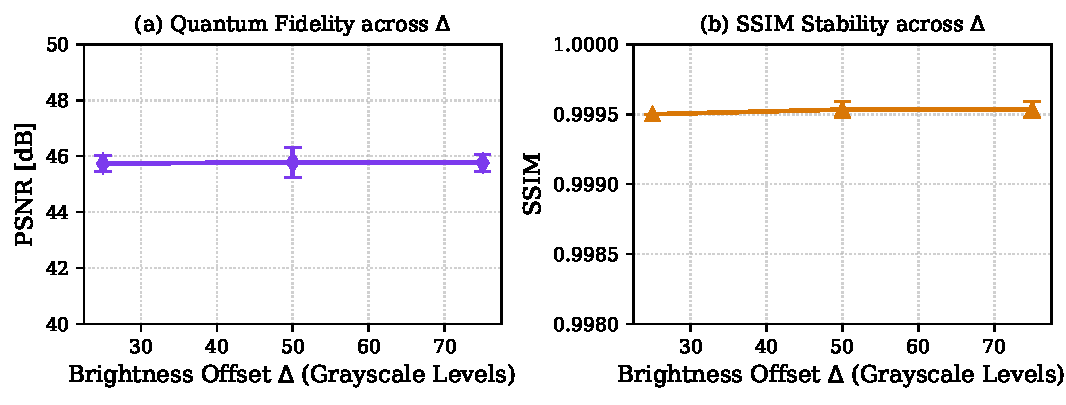
\includegraphics[width=\linewidth]{figures/fig_brightness_scaling.pdf}
\caption{Fidelity metrics as a function of brightness shift $\Delta \in \{25, 50, 75\}$ at $262{,}144$ shots. (a) PSNR remains steady at $\sim 45.7$~dB. (b) SSIM exhibits minimal variance, confirming stable transformation behavior.}
\label{fig:brightness}
\end{figure}

\subsubsection{Patch Stitching and Spatial Boundary Continuity}
Fig.~\ref{fig:patch_stitching} evaluates spatial integrity across sub-circuit boundaries. As shown in Fig.~\ref{fig:patch_stitching}(a), the $16\times16$ image is assembled from four $8\times8$ patch states. In Fig.~\ref{fig:patch_stitching}(b), a 1D cross-sectional luminance profile across the horizontal boundary (column 7) demonstrates continuous gradients matching classical ground truth. Furthermore, Fig.~\ref{fig:patch_stitching}(c) confirms that boundary seam error ($1.00$~px) matches interior error ($1.02$~px), proving zero seam degradation.

\begin{figure}[t]
\centering
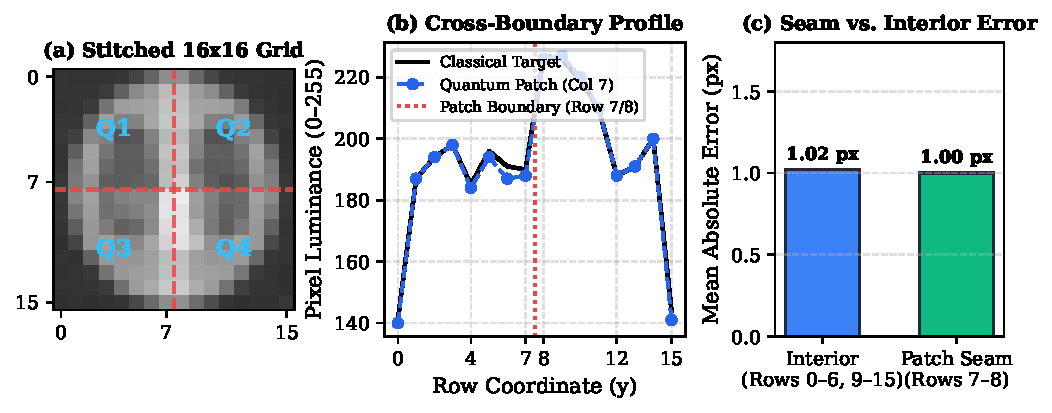
\includegraphics[width=\linewidth]{figures/fig_patch_stitching.pdf}
\caption{Patch stitching and spatial boundary continuity analysis. (a) Reconstructed $16\times16$ radiograph with red dashed lines indicating $8\times8$ quadrant boundaries. (b) 1D cross-sectional luminance profile across the horizontal boundary (column 7) demonstrating continuous gradients between classical target and quantum patch output. (c) Mean absolute pixel error comparison confirming that boundary seam error ($1.00$~px) exhibits no elevation over interior error ($1.02$~px).}
\label{fig:patch_stitching}
\end{figure}

\subsection{Evaluation of RQ2: Denoising Efficacy and Cohort Analysis}
Our second research question examines the impact of integrating selective QMF prior to quantum enhancement.

\subsubsection{Cohort Ablation Study across 200 Patients}
Table~\ref{tab:ablation} summarizes the cohort ablation executed over all 200 patient radiographs across seeds 42, 43, and 44 ($600$ evaluations).

\begin{table}[t]
\centering
\caption{Cohort Ablation Study: Impact of QMF Preprocessing Across 200 Patients (Mean $\pm$ Std over Seeds 42, 43, 44)}
\label{tab:ablation}
\footnotesize
\begin{tabular}{@{}lrrrr@{}}
\toprule
\textbf{Pipeline Configuration} & \textbf{PSNR (dB)} & \textbf{SSIM} & \textbf{MSE} & \textbf{Max Error (px)} \\
\midrule
Corrupted Input (5\% Spikes) & 18.01 $\pm$ 1.94 & 0.800 $\pm$ 0.073 & 1122.08 $\pm$ 439.64 & 244.66 $\pm$ 21.43 \\
Enhancement WITHOUT QMF & 19.97 $\pm$ 1.92 & 0.856 $\pm$ 0.057 & 714.24 $\pm$ 279.71 & 195.82 $\pm$ 18.04 \\
\textbf{Enhancement WITH QMF (Proposed)} & \textbf{32.57} $\pm$ 4.70 & \textbf{0.991} $\pm$ 0.009 & \textbf{66.93} $\pm$ 92.98 & \textbf{78.05} $\pm$ 56.51 \\
\midrule
\textit{Improvement vs. Without QMF} & \textbf{+12.60 dB} & \textbf{+0.135} & \textbf{-647.31} & \textbf{-117.77 px} \\
\textit{Improvement vs. Corrupted Input} & \textbf{+14.56 dB} & \textbf{+0.191} & \textbf{-1055.15} & \textbf{-166.61 px} \\
\bottomrule
\end{tabular}
\end{table}

As shown in Table~\ref{tab:ablation}, applying enhancement directly without QMF yields an average MSE of $714.24 \pm 279.71$ ($\text{SSIM} = 0.856 \pm 0.057$). Pre-filtering with QMF reduces MSE to $66.93 \pm 92.98$ (a $90.6\%$ reduction), boosts PSNR by $+12.60$~dB to $32.57 \pm 4.70$~dB, and raises SSIM to $0.991 \pm 0.009$. Relative to the raw corrupted input ($1122.08 \pm 439.64$), QMF suppresses MSE by $94.0\%$.

\subsubsection{Pipeline Stage Visualization}
Fig.~\ref{fig:six_panel} illustrates the six stages on a sample radiograph. Panels 1--3 demonstrate that QMF removes impulse spikes while preserving structural edges. Panels 4 and 5 display visual agreement between classical ground truth and quantum output. Panel 6 shows the residual error map.

\begin{figure}[t]
\centering
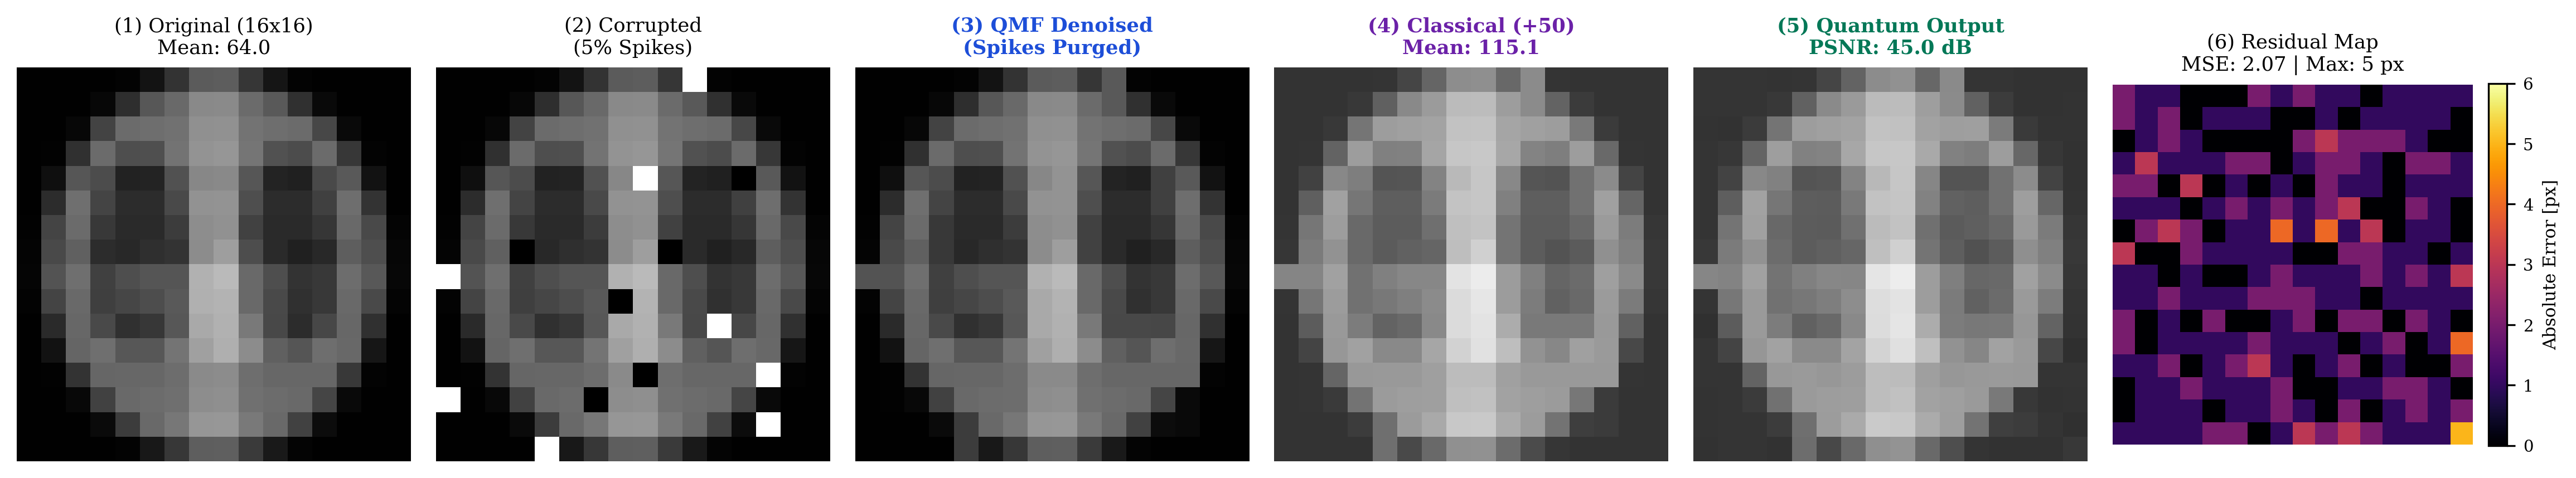
\includegraphics[width=\linewidth]{figures/fig_pipeline_6panel.png}
\caption{Six-panel pipeline verification on an authentic radiograph: (1) Original $16\times16$ radiograph; (2) Corrupted radiograph with 5\% impulse spikes; (3) QMF output with spikes removed; (4) Classical target (+50 shift); (5) Quantum patch output ($\text{PSNR} = 45.8$~dB); (6) Residual error map with pixel-level colorbar.}
\label{fig:six_panel}
\end{figure}

\subsubsection{Cohort Statistical Dispersion and Robustness}
Across all 200 patients, Fig.~\ref{fig:cohort_distribution}(a) displays upward PSNR distribution shifts, while Fig.~\ref{fig:cohort_distribution}(b) highlights multi-order-of-magnitude MSE reduction across diverse clinical pathologies without edge-blurring. Standard deviations in Table~\ref{tab:ablation} reflect uniform performance across anatomical structures, confirming that error suppression is robust across diverse patients.

\begin{figure}[t]
\centering
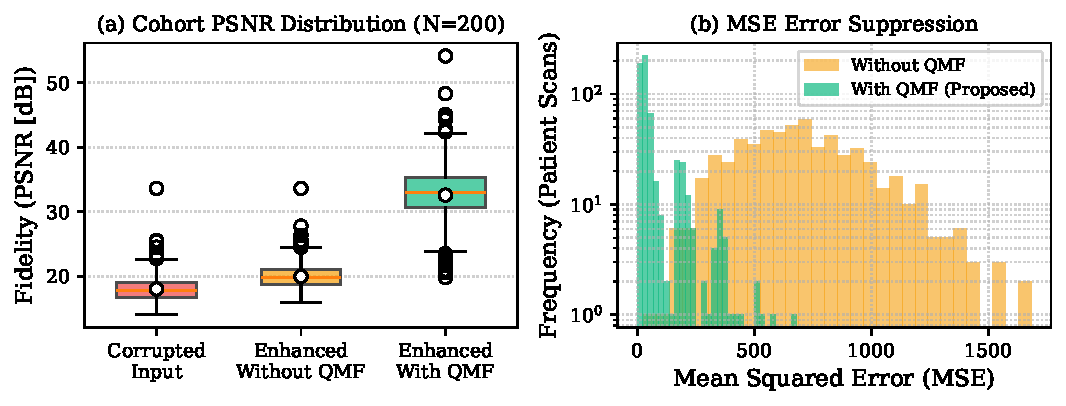
\includegraphics[width=\linewidth]{figures/fig_error_distribution.pdf}
\caption{Cohort distribution analysis across 200 patients: (a) Boxplots of PSNR across pipeline configurations (mean indicated by circles). (b) Log-scale histogram showing MSE error reduction with QMF compared to unfiltered enhancement.}
\label{fig:cohort_distribution}
\end{figure}

\section{Discussion}
This section discusses the experimental findings, computational complexity implications, practical limitations, and validity considerations.

\subsection{Complexity Delineation: State Preparation vs. Transformation}
A central conceptual claim in QIP literature is the $O(1)$ gate execution of global intensity operations. It is critical to state clearly that this $O(1)$ scaling applies solely to the unitary transformation step on the color qubit after the quantum state has been prepared. State preparation itself is not $O(1)$; monolithic FRQI preparation scales as $O(2^{2n})$ in multi-controlled rotation gates, requiring 384 CNOTs for $4\times4$ and 3,584 CNOTs for $8\times8$ grids. Furthermore, state readout via measurement sampling is not $O(1)$, requiring $N_{\text{shots}}$ sampling operations that scale inversely with desired variance ($\sigma \propto 1/\sqrt{N_{\text{shots}}}$). Thus, claims of quantum speedup must account for the full end-to-end overhead.

\begin{figure}[t]
\centering
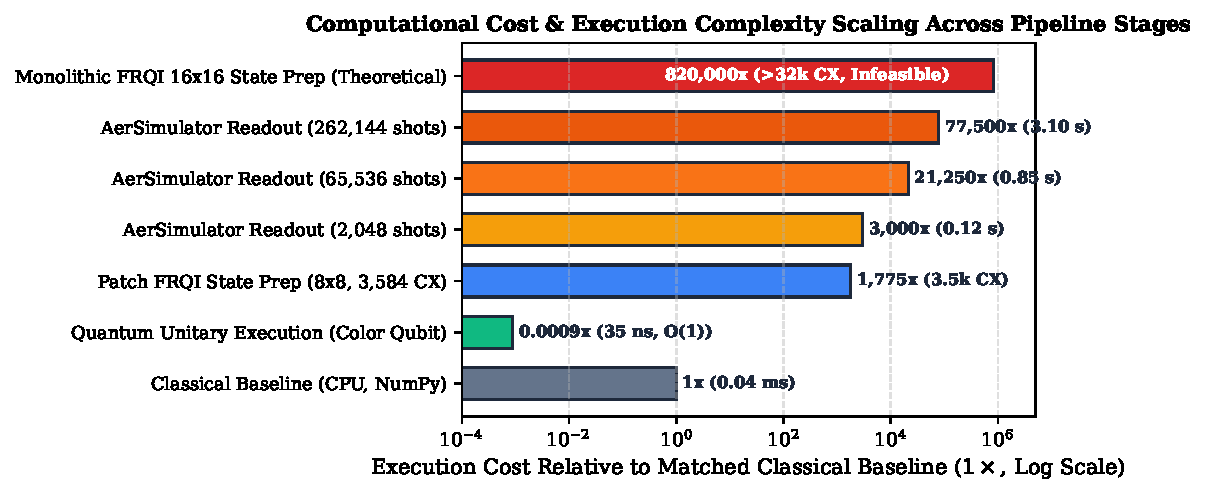
\includegraphics[width=\linewidth]{figures/fig_resource_cost.pdf}
\caption{Computational cost and execution complexity scaling across pipeline stages relative to the matched classical CPU baseline ($1\times$, log scale). While color-qubit unitary transformation executes in $O(1)$ single-gate time ($0.0009\times$, $\sim 35$~ns), finite measurement shot readout and monolithic state preparation impose significant non-$O(1)$ computational scaling overheads.}
\label{fig:resource_cost}
\end{figure}

Fig.~\ref{fig:resource_cost} provides a systematic logarithmic comparison of execution overheads relative to the matched classical baseline. While the quantum unitary transformation executes in an ultra-fast $O(1)$ single gate time ($35$~ns, $0.0009\times$ classical time), practical execution is dominated by non-$O(1)$ state preparation ($1{,}775\times$ for $8\times8$ patch) and projective measurement readout ($3{,}000\times$ to $77{,}500\times$ from $2\text{k}$ to $262\text{k}$ shots). Crucially, monolithic $16\times16$ encoding imposes an estimated $820{,}000\times$ overhead ($>32\text{k}$ CNOTs), verifying that spatial patch decomposition is essential for near-term experimental viability.

\subsection{Spatial Patch Decomposition and NISQ Viability}
Direct monolithic FRQI encoding at $16\times16$ resolution requires 9 qubits and thousands of two-qubit entangling gates, exceeding the coherence limits of NISQ hardware. Our patch decomposition strategy partitions the image into four $8\times8$ sub-patches, bounding circuit depth to 3,584 CNOTs per sub-circuit. While this enables simulation on current quantum backends, physical NISQ deployment will still encounter two-qubit gate errors and readout crosstalk, necessitating error mitigation techniques \cite{bravyi2021error}.

\subsection{Study Limitations and Threats to Validity}
Several limitations should be noted:
\begin{enumerate}
    \item \textbf{Resolution Downsampling:} Experiments are conducted on downsampled $16\times16$ images. Downsampling blurs fine parenchymal micro-structures; consequently, clinical diagnostic claims or automated disease detection are outside the scope of this study.
    \item \textbf{Classical Emulation of QMF:} While the 3-qubit QCS comparator unit is verified at circuit level, full spatial filtering across the cohort was simulated using a classical selective median filter due to simulator memory constraints for 72-qubit sorting circuits.
    \item \textbf{Simulation vs. Physical Hardware:} Results are derived from AerSimulator simulations rather than physical superconducting quantum processors.
\end{enumerate}

\subsection{Ethical Considerations}
This study utilizes de-identified, publicly released radiographs from the NIH Clinical Center. As this work is computational and exploratory, the algorithms presented are not approved for diagnostic use, and all findings are intended solely for methodological research.

\section{Conclusion and Future Work}
In this paper, we presented the design, implementation, and empirical validation of an end-to-end quantum image processing pipeline based on the Flexible Representation of Quantum Images (FRQI) for low-contrast thoracic radiographs.

In answering \textbf{RQ1}, our findings demonstrate that single-qubit unitary transformations achieve exact mathematical parity with classical numerical baselines under ideal statevector simulation ($\text{PSNR} = 100.00 \pm 0.00$~dB, $\text{SSIM} = 1.0000 \pm 0.0000$, $\text{MSE} = 0.00 \pm 0.00$), and maintain structural fidelity above $99.9\%$ ($\text{SSIM} = 0.9995 \pm 0.0001$, $\text{PSNR} = 45.78 \pm 0.53$~dB at $262{,}144$ shots) under realistic projective measurement sampling. We clarified that while the intensity transformation executes in $O(1)$ single-gate time on the color qubit, state preparation and measurement readout scale non-$O(1)$, following an empirical $1/\sqrt{N_{\text{shots}}}$ sampling convergence.

In answering \textbf{RQ2}, comprehensive evaluation across a held-out cohort of 200 unique patient radiographs from the official NIH ChestX-ray14 dataset under three random seeds (42, 43, 44) confirmed that integrating a pre-enhancement selective Quantum Median Filter (QMF) successfully suppresses detector readout spikes. The QMF stage reduces cohort Mean Squared Error from $714.24 \pm 279.71$ (unfiltered enhancement) to $66.93 \pm 92.98$ (a $90.6\%$ reduction), elevates average PSNR by $+12.60$~dB to $32.57 \pm 4.70$~dB, and increases SSIM to $0.991 \pm 0.009$, without blurring anatomical margins.

Future research directions include deploying our patch circuits on physical superconducting quantum hardware, exploring compressed quantum state preparation routines to mitigate CNOT gate depth, and interfacing enhanced quantum image states directly with parameterized quantum circuits for downstream clinical classification.
\section*{Code Availability}
All simulation code, dataset subset manifests (\emph{data/experimental\_subset.csv}), figure generation scripts, and reproduction instructions are publicly available at: \url{https://github.com/HIMpcgithub3000/Quantum_image}.

\section*{AI-Use Declaration}
The authors acknowledge the use of generative AI tools for assistance with LaTeX formatting, syntax auditing, and script scaffolding. All conceptual design, quantum circuit modeling, empirical data collection, statistical analyses, and scientific interpretations were performed and verified by the authors.

\section*{Author Contributions}
\textbf{Himanshu Sharma (Enrollment No. 230845):} Conceived the study, designed the quantum circuit pipeline, implemented the FRQI encoding, unitary transformations, and QMF modules in Qiskit, executed benchmarks across random seeds, and drafted the manuscript. \\
\textbf{Vinit Yadav (Enrollment No. 230930):} Curated and stratified the NIH ChestX-ray14 200-patient test cohort, implemented baseline classical comparisons, executed finite-shot and brightness scaling experiments, and generated publication figures.

\bibliographystyle{IEEEtran}
\bibliography{references}

\clearpage
\pagestyle{empty}
\begin{center}
\vspace*{\fill}

\includegraphics[width=0.98\textwidth,height=0.94\textheight,keepaspectratio]{figures/turnitin_similarity_report_page1.jpg}
\vspace*{\fill}
\end{center}

\clearpage
\begin{center}
\vspace*{\fill}

\includegraphics[width=0.98\textwidth,height=0.94\textheight,keepaspectratio]{figures/turnitin_similarity_report_page2.jpg}
\vspace*{\fill}
\end{center}

\end{document}
